\let\negmedspace\undefined
\let\negthickspace\undefined
\documentclass[journal]{IEEEtran}
\usepackage[a5paper, margin=10mm, onecolumn]{geometry}
%\usepackage{lmodern} % Ensure lmodern is loaded for pdflatex
\usepackage{tfrupee} % Include tfrupee package

\setlength{\headheight}{1cm} % Set the height of the header box
\setlength{\headsep}{0mm}     % Set the distance between the header box and the top of the text

\usepackage{gvv-book}
\usepackage{gvv}
\usepackage{cite}
\usepackage{amsmath,amssymb,amsfonts,amsthm}
\usepackage{algorithmic}
\usepackage{graphicx}
\usepackage{textcomp}
\usepackage{xcolor}
\usepackage{txfonts}
\usepackage{listings}
\usepackage{enumitem}
\usepackage{mathtools}
\usepackage{gensymb}
\usepackage{comment}
\usepackage[breaklinks=true]{hyperref}
\usepackage{tkz-euclide} 
\usepackage{listings}
% \usepackage{gvv}                                        
\def\inputGnumericTable{}                                 
\usepackage[latin1]{inputenc}                                
\usepackage{color}                                            
\usepackage{array}                                            
\usepackage{longtable}                                       
\usepackage{calc}                                             
\usepackage{multirow}                                         
\usepackage{hhline}                                           
\usepackage{ifthen}                                           
\usepackage{lscape}
\begin{document}

\bibliographystyle{IEEEtran}
\vspace{3cm}

\title{1.1.6.9}
\author{EE24BTECH11030 - J.KEDARANANDA
}
% \maketitle
% \newpage
% \bigskip
{\let\newpage\relax\maketitle}

\renewcommand{\thefigure}{\theenumi}
\renewcommand{\thetable}{\theenumi}
\setlength{\intextsep}{10pt} % Space between text and floats


\numberwithin{equation}{enumi}
\numberwithin{figure}{enumi}
\renewcommand{\thetable}{\theenumi}


\textbf{Question}:\\
If three points $\brak{h,0}$,$\brak{a,b}$ and $\brak{0,k}$ lie on a line, show that \\
$\frac{a}{h} + \frac{b}{k} = 1$\\

\textbf{Solution: }
\begin{table}[h!]    
  \centering
  \begin{center}
    \begin{tabular}{|c|c|} 
        \hline
            \textbf{Variable} & \textbf{Value} \\ 
        \hline
            $\boldsymbol{BC}$ & 6 cm \\ 
        \hline
            $\boldsymbol{AB}$ & 5 cm \\ 
        \hline
            $\angle \vec{B}$  & $60^\circ$ \\
        \hline
    \end{tabular}
\end{center}  



  \caption{Variables Used}
  \label{tab10.5.3.9.1}
\end{table}\\
As given points lie on same line its determinant value should be equal to 0.
\begin{align}
 \mydet {h & 0 & 1 \\ a & b & 1 \\ 0 & k & 1} = 0 \label{1.6.9.1}
\end{align}
expanding the det by column 3.
\begin{align}
 1\mydet {h & 0 \\ a & b} - 1\mydet{ h & 0 \\ 0 & k } + 1\mydet { a & b \\ 0 & k } = 0
\end{align}
\begin{align}
 hb - hk + ak = 0
\end{align}
\begin{align}
 \frac{hb}{hk} - \frac{hk}{hk} + \frac{ak}{hk} = 0
\end{align}
\begin{align}
 \frac{b}{k} + \frac{a}{h} = 1
\end{align}
\textbf{EXAMPLE}\\
lets take 3 points as an example and check whether they follow our line equation or not \\
(2,0)(1,2)(0,4)
\begin{align}
 \frac{a}{h} + \frac{b}{k} = 1
\end{align}
\begin{align}
 \frac{1}{2} + \frac{2}{4}  =  1
\end{align}
these points satisfy our line equation
\begin{figure}[h!]
   \centering
   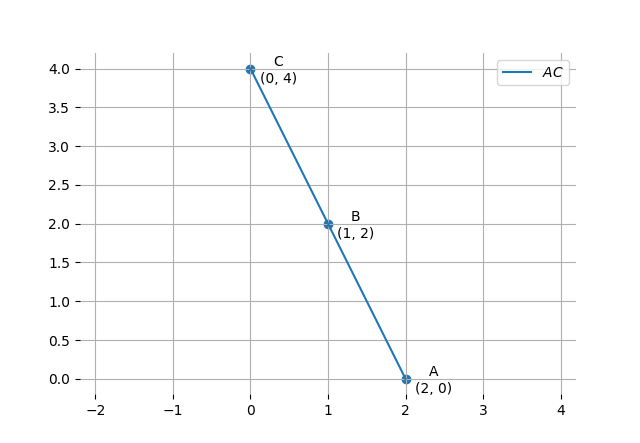
\includegraphics[width=0.7\linewidth]{figs/fig2.png}
   \caption{Stem Plot of y\brak{n}}
   \label{stemplot}
\end{figure}
\end{document}  
\end{document}
